\chapter{Replico}\label{chap:method}

    % todo: cite wim
    After evaluating the literature, there appears to be a promising avenue for exploring a method for DeskVR users to engage in discussions and communicate about various objects and areas of interest within a shared virtual environment. This approach could enhance communication effectiveness, especially considering the challenges associated with verbally referencing objects and describing spatial locations \cite{odaVirtualReplicasRemote2015}. Moreover, given the unique constraints of DeskVR, a research gap exists in applying such methods to this specific environment. Thus, this work introduces Replico, a collaborative touch-based DeskVR approach that utilizes the world-in-miniature (WIM) \cite{stoakleyVirtualRealityonaWim1995} metaphor to facilitate reasoning about 3D models.

\section{Overview} \label{sec:overview}

    After recognizing the potential of a collaborative DeskVR approach to enhance communication and reasoning about 3D models, it became important to outline the basic needs such an approach should meet. These requirements stem from the desire to address common challenges faced by users in virtual environments, aligning with DeskVR's goals of minimizing physical effort to enable longer periods of productive work, reducing mistakes to prevent frustration, and getting more done in less time. Additionally, the approach should be easy to understand to facilitate seamless collaboration with others and allow users to communicate effectively about objects and areas of interest even when they are out of sight.

    Furthermore, users must know where others are, who they are, and what they are doing in the virtual space to work well together. Users should be able to easily determine the location and activities of their counterparts so they can coordinate and talk effectively. Importantly, all interactions and tasks should be achievable while seated so they can keep working without getting too tired.

    To meet these needs, the chosen approach utilizes the world-in-miniature (WIM) metaphor \cite{stoakleyVirtualRealityonaWim1995}. The WIM is a miniature replica of the virtual environment that can be easily manipulated within arm's reach and viewed from multiple angles, making it a good fit for DeskVR. Changes made in the miniature model are reflected in the full-scale model. Additionally, the WIM is effective for displaying social information, such as users' locations and where they are looking, as well as indicating who is working. Each user has a personal view of the WIM, while the to-scale model is shared.

    The approach allows users to create points of interest to facilitate communication about objects and zones of interest. These points are uniquely identified by a number and an appearance corresponding to their owner. For instance, one user's points of interest might be represented by green striped spheres, while purple checkerboard cubes represent another user's points. These points of interest are visible in both the to-scale 3D model and its WIM counterpart and remain visible even if occluded.

    Users are attached to virtual tables that correspond to their real-life counterparts. They can either remain at separate tables or join another user's table to share the same point of view of the to-scale model. Users can also teleport around the 3D model, taking their table with them if they are alone or creating a new one if they are at someone else's table.

    To reduce physical effort, the approach uses touch-based gestures for interactions, such as moving the replica and creating points of interest. Literature suggests that touch-based interactions help reduce physical strain and increase comfort \cite{benkoBalloonSelectionMultiFinger2007, almeidaSIT6IndirectTouchbased2023}. Specifically, the approach incorporates the Balloon Selection metaphor \cite{benkoBalloonSelectionMultiFinger2007} for creating points of interest. Balloon Selection was chosen mainly due to its "\textit{String Height Clutching}" feature, which allows users to increase the height of the selection cursor infinitely. This is in contrast to the Triangle Cursor \cite{strothoffTriangleCursorInteractions2011}, and it is less straining than Corkscrew Selection \cite{daiberBalloonSelectionRevisited2012}, which requires rotational movement.

    %\begin{figure}
    %    \centering
    %    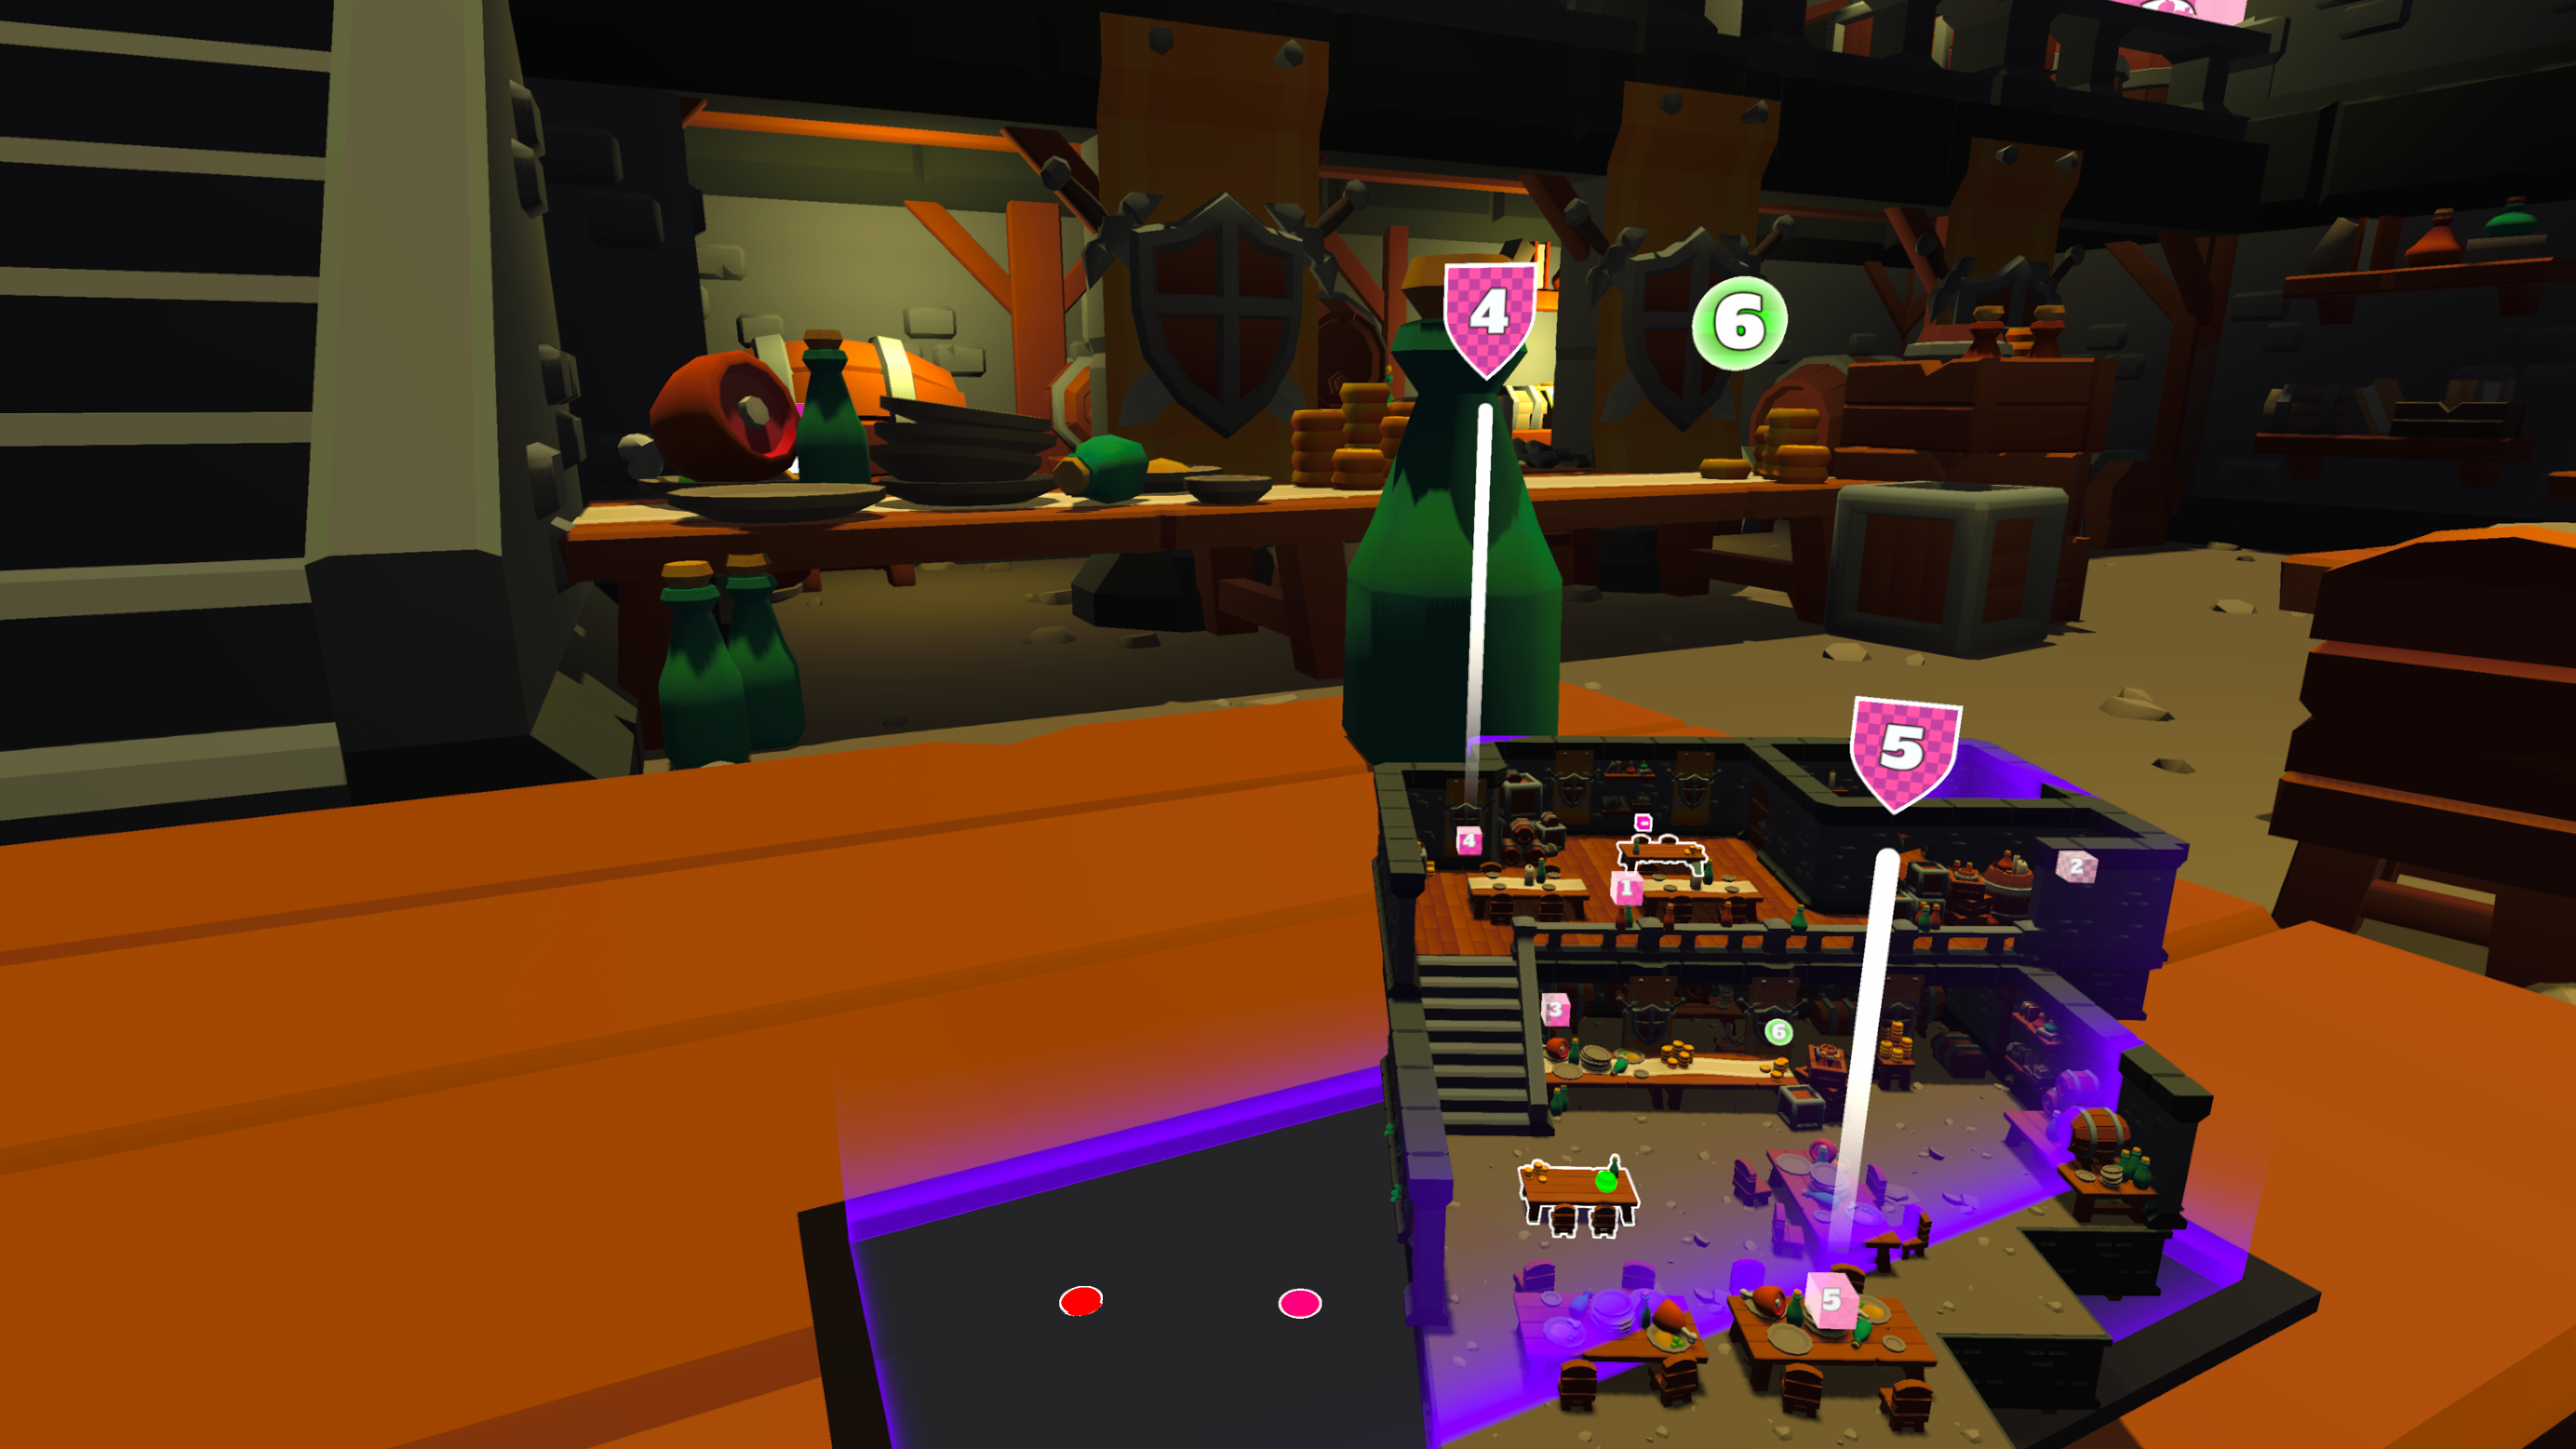
\includegraphics[width=1\linewidth]{figures/description.png}
    %    \caption{Usage example of the approach from the implemented prototype. This figure shows various elements: a virtual representation %of the user's table, a representation of the touch frame and active fingers, points of interest, and user locations.}
    %    \label{fig:description}
    %\end{figure}
    
\section{Actions} \label{sec:actions}

    This section details the specific actions users can perform within Replico using touch-based gestures. These actions encompass various interactions and transformations. Similar to Balloon Selection \cite{benkoBalloonSelectionMultiFinger2007}, these gestures are handedness-agnostic, meaning they can be performed with either the left or right hand. The following subsections outline the key actions and how to perform them.

    \subsection{Replica Transformations} \label{sec:transform}

        Transformations to the replica closely resemble the common gestures associated with touch screens on mobile phones for zooming, panning, and rotating images. Translation in the XZ plane is done by placing one or more fingers on the touch table and moving them. Yaw rotation around the Y-axis is achieved by rotating the fingers around the center of their positions, which also serves as the center of rotation. Scaling the replica in all dimensions is accomplished using a pinch gesture, with the scaling base centered on the midpoint of the fingers and the WIM's base y position.

        Translation along the Y-axis is achieved by first placing a finger from the primary hand on the table, followed by two fingers from the secondary hand. The fingers of the secondary hand control translation on the XY plane, while the fingers of the primary hand can perform all the previously mentioned transformations.

        % I have to put in here some images, not sure what

    \subsection{Balloon Selection} \label{sec:balloon}

        Replico uses the Balloon Selection metaphor \cite{benkoBalloonSelectionMultiFinger2007} to create, delete, and acknowledge points of interest, as well as teleportation, and join another user's table. To initiate the balloon selection gesture, the user places a finger from their primary hand on the table, followed by a finger from their secondary hand. This action brings up a balloon on the user's table relative to the WIM, with a copy visible on the to-scale 3D model. The primary finger controls the XZ position of the balloon while moving the fingers apart lowers the balloon, and bringing them together raises it. Users can remove the secondary finger without changing the balloon's height, allowing for "String Height Clutching."
    
        To perform a \textit{selection}, the user briefly adds a second finger from their secondary hand to the touch table. This \textit{selection} action can create points of interest at the balloon's position, delete points of interest if the balloon intersects with one of the user's points, acknowledge points of interest if the balloon intersects another user's unacknowledged points, and join other users' tables if it intersects another user's table.
    
        For \textit{teleportation}, the user similarly adds a second finger from their secondary hand to the touch table but holds it in place until an arrow appears on the balloon, indicating the teleportation's end orientation. To rotate the balloon, the user performs a gesture similar to the replica's rotation gesture by rotating their fingers around their midpoint. Either hand can be removed to reposition, but removing both hands cancels the teleportation. To confirm the teleportation, the user taps again with the second finger of the secondary hand.


\section{Awareness} \label{sec:awareness}

    Following Table \ref{tab:workspaceElementsPast}, Replico incorporates most elements of workspace awareness. Users have distinct appearances that uniquely identify them, which is also reflected in their points of interest, albeit with some distinguishing features. User tables are represented in the WIM by outlined miniatures, positioned and oriented as they are in the to-scale model, and are visible behind objects. These miniature tables display who is at each table through miniature representations of the users.
    
    Points of interest created by other users are initially in an \textit{unacknowledged} state, marked by a vertical line capped with a symbol that resembles the owner's appearance and includes the balloon's identification number. This system, combined with the acknowledgment gesture described in \ref{sec:balloon}, allows users to distinguish recently created points of interest from previously created ones.
    
    These representations blend abstract and mimetic representations of social information as described in \cite{ericksonSocialTranslucenceApproach2000}. They are mimetic in representing real-world entities like tables and user avatars, yet abstract as they are symbolic and easy to create and manipulate.
    
    Thus, Replico allows users to ascertain the presence of others in the workspace, their locations, and their viewing directions by observing the tables in the replica. Users can identify others by their appearance, determine collaborators by noting who shares the same table, and discern authorship through the appearance of points of interest. Points of interest, in turn, indicate which objects users are working on. Additionally, users can track recent activities by checking unacknowledged points.

\section{Summary}
    This chapter introduces Replico, a collaborative DeskVR approach designed to enhance communication and interaction in the analysis of 3D models. Using the world-in-miniature (WIM) metaphor, Replico addresses common challenges in virtual collaboration, such as spatial referencing and awareness of other users' activities.

    First, it explains the requirements such an approach should consider, such as minimizing physical effort, reducing mistakes, ensuring efficiency, effective communication about objects and areas of interest, ease of understanding, providing awareness of other users, and enabling all interactions to be done while seated. To meet these requirements, Replico allows users to manipulate a miniature replica of the virtual environment (WIM). This approach ensures that changes made in the miniature are reflected in the full-scale model. Replico also enables the creation of uniquely identified points of interest, aiding the communication about objects and zones of interest within the virtual space. Users are attached to virtual tables corresponding to their real-life counterparts, allowing them to join others' tables or teleport around the 3D model.

    Section \ref{sec:actions} explains the different touch-based gestures users can perform within Replico: translation, rotation, and scaling of the WIM; and creation, deletion, and acknowledgment of points of interest, as well as teleportation and joining users' tables, using balloon selection. Section \ref{sec:awareness} explains how Replico incorporates workspace awareness: users and their points of interest share a unique appearance, making them identifiable; user tables are represented in the replica; and points of interest can be acknowledged to identify recent points of interest quickly.